\documentclass[a4paper,11pt]{article}

% ==========================================
% 1. CONFIGURACIÓN DEL PROYECTO
% ==========================================
\newcommand{\titol}{Aprendizaje no supervisado y detección de anomalías}
\newcommand{\subtitol}{Documento de descripción de los problemas de la exposición}
\newcommand{\assignatura}{Computació d'Altes Prestacions i Intel·ligència Artificial (CPIA)}
\newcommand{\assignaturaCurt}{CPIA (UPC)}
\newcommand{\universitat}{Universitat Politècnica de Catalunya}
\newcommand{\escola}{ETSETB / FIB}
\newcommand{\autorA}{Matías, Martí, Uriel y Arnau Montull}
\newcommand{\autorB}{Grado en Ingeniería Física}

% ==========================================
% 2. PAQUETES Y CONFIGURACIÓN TIPOGRÁFICA
% ==========================================
\usepackage[utf8]{inputenc}
\usepackage[T1]{fontenc}
\usepackage{lmodern}
\usepackage[spanish,es-nodecimaldot]{babel}

% Estandarizar nombre de tablas
\addto\captionsspanish{\renewcommand{\tablename}{Tabla}}

\usepackage{amsmath, amssymb, amsfonts, amsthm}
\usepackage{mathtools}
\usepackage{geometry}
\geometry{
    left=2.1cm,
    right=2.1cm,
    top=2.2cm,
    bottom=2.2cm,
    headheight=14.5pt
}

\usepackage{microtype}
\usepackage{graphicx}
\usepackage{parskip}   
\usepackage{caption}
\usepackage{subcaption} 
\usepackage{fancyhdr}   
\usepackage{xcolor}
\usepackage{booktabs}
\usepackage{tabularx}  
\usepackage{array}
\usepackage{siunitx}
\sisetup{output-decimal-marker = {.}}

% Control fino de distancias para figuras flotantes
\setlength{\textfloatsep}{10pt plus 2pt minus 2pt}
\setlength{\intextsep}{9pt plus 2pt minus 2pt}
\setlength{\floatsep}{8pt plus 2pt minus 2pt}

% Hipervínculos
\usepackage{hyperref}
\hypersetup{
    colorlinks=true,
    linkcolor=blue!70!black,
    citecolor=green!50!black,
    urlcolor=blue!80!black
}

% Cabeceras y pies de página
\pagestyle{fancy}
\fancyhf{}
\lhead{\small \textbf{\assignaturaCurt}}
\rhead{\small \autorA, \autorB}
\cfoot{\small \thepage}
\renewcommand{\headrulewidth}{0.4pt}

% Configuración para código fuente
\usepackage{listings}
\definecolor{mGreen}{rgb}{0,0.55,0}
\definecolor{mGray}{rgb}{0.45,0.45,0.45}
\definecolor{mPurple}{rgb}{0.55,0,0.75}
\definecolor{codeBackground}{rgb}{0.97,0.98,0.99}

\lstset{
    language=Python,
    backgroundcolor=\color{codeBackground},   
    commentstyle=\color{mGreen}\itshape,
    keywordstyle=\color{blue}\bfseries,
    numberstyle=\tiny\color{mGray},
    stringstyle=\color{mPurple},
    basicstyle=\ttfamily\footnotesize, 
    breakatwhitespace=false,         
    breaklines=true,                 
    captionpos=b,                    
    keepspaces=true,                 
    numbers=left,                    
    numbersep=8pt,                  
    tabsize=2,
    frame=single,                    
    rulecolor=\color{black!15},
    xleftmargin=16pt,
    framexleftmargin=6pt
}

% ==========================================
% 3. INICIO DEL DOCUMENTO
% ==========================================

% ---- extras de este documento ----
\lstset{language=Python, inputencoding=utf8, extendedchars=true,
  literate={á}{{\'a}}1 {é}{{\'e}}1 {í}{{\'i}}1 {ó}{{\'o}}1 {ú}{{\'u}}1 {ñ}{{\~n}}1 {Á}{{\'A}}1 {°}{{$^\circ$}}1 {–}{{--}}1 {—}{{---}}1}
\usepackage{float}
\newcommand{\pendiente}[1]{\textcolor{red!70!black}{\textbf{[PENDIENTE: #1]}}}

\begin{document}

% --- PORTADA ---
\begin{titlepage}
    \thispagestyle{empty}
    \centering
    \vspace*{0.2cm}
    
\includegraphics[width=0.16\textwidth]{Logo_UPC.svg.png}\\[0.3cm]
    {\large \textbf{\universitat}}\\[0.12cm]
    {\normalsize \escola}\\[0.9cm]
    \rule{\textwidth}{0.6pt}\\[0.35cm]
    {\LARGE \textbf{\titol}}\\[0.25cm]
    {\large \subtitol}\\[0.15cm]
    \rule{\textwidth}{0.6pt}\\[0.7cm]
    {\large \textbf{\assignatura}}\\[0.45cm]
    {\large \textbf{Equipo:}}\\[0.12cm]
    {\large \autorA}\\[0.08cm]
    {\large \autorB}\\[1.2cm]
    \vfill
    
\includegraphics[width=0.12\textwidth]{logo-enginyeria-fisica.jpg}\\[0.25cm]
    {\normalsize \today}
\end{titlepage}

\clearpage

\tableofcontents
\clearpage

% ==========================================
\section{Equipo y reparto de problemas}
% ==========================================
Exposición del tema «Aprendizaje no supervisado y detección de anomalías». El objetivo es entender cómo encontrar
estructura y patrones en datos sin etiquetar con clustering (K-Means, DBSCAN, jerárquico), mezclas gaussianas e
Isolation Forest, y cómo evaluar un clustering sin etiquetas (silhouette y método del codo).

\begin{table}[H]
\centering
\begin{tabularx}{\textwidth}{@{}l>{\raggedright\arraybackslash}X>{\raggedright\arraybackslash}Xl@{}}
\toprule
Integrante & Problema & Algoritmo principal & Fichero \\
\midrule
Arnau Montull & Detección de explosiones nucleares entre sismos (catálogo USGS) & DBSCAN (haversine) & \texttt{nukeDBSCAN\_arnau.py} \\
Matías & Agrupación de sismos del último mes y detección de anomalías & K-Means ($K=3$) y $k$-vecinos más próximos & \texttt{presentation\_matias.py}, \texttt{validacio.py} \\
Martí & Transcriptómica (RNA-seq): módulos de genes co-expresados y muestras anómalas & Clustering jerárquico, K-Means, DBSCAN, Isolation Forest & \pendiente{fichero \texttt{.py} (aún sin código)} \\
Uriel & \pendiente{título del problema} & \pendiente{algoritmo} & \pendiente{fichero} \\
\bottomrule
\end{tabularx}
\caption{Reparto de problemas. Cada fichero se llama \texttt{<nemotécnico>\_<estudiante>.py}.}
\end{table}

\section{Fundamentos comunes}
Resumen de los conceptos que usan los problemas. La explicación completa de K-Means (en catalán) está en
\texttt{docs/teoria/fonaments\_de\_clustering\_i\_kmeans.tex}.

\paragraph{Aprendizaje no supervisado y clustering.} Se busca estructura en datos sin etiquetas. Cada algoritmo
necesita una medida de similitud (distancia euclídea, haversine, correlación\ldots) y la elección condiciona el resultado.

\paragraph{K-Means.} Divide los datos en $K$ grupos minimizando la suma de distancias cuadráticas de cada punto al centroide
de su grupo, $J=\sum_{k=1}^{K}\sum_{x\in C_k}\lVert x-\mu_k\rVert^2$. Se resuelve con el algoritmo de Lloyd (asignar cada punto
al centroide más cercano y recalcular centroides, hasta converger), inicializado con $K$-means++. Es un clustering \emph{duro}, supone grupos
compactos y de tamaño parecido, y hay que fijar $K$.

\paragraph{Cómo elegir $K$ sin etiquetas.} Método del codo (la inercia deja de bajar de forma apreciable), coeficiente de
silueta, $s=(b-a)/\max(a,b)$, con $a$ la distancia media a los puntos de su grupo y $b$ la distancia media al grupo vecino más
próximo, e índice de Davies--Bouldin.

\paragraph{DBSCAN.} Agrupa por densidad: un punto es \emph{central} si tiene al menos $v_{\min}$ puntos (él incluido) a
distancia $\le\varepsilon$; los grupos son las componentes conexas de puntos centrales y los puntos que no alcanza ninguno
quedan como ruido ($-1$). No necesita fijar el número de grupos y encuentra formas arbitrarias.

\paragraph{Clustering jerárquico, mezclas gaussianas e Isolation Forest.} El jerárquico construye un dendrograma según
el tipo de enlace (simple, medio, Ward) y se corta a una altura. Las mezclas gaussianas (\texttt{GaussianMixture}) dan una asignación
blanda por probabilidad. Isolation Forest puntúa como anómalos los puntos que se aíslan con pocos cortes aleatorios.
\pendiente{el equipo revisa y amplía este resumen con lo que se exponga.}

% ==========================================
\section{Problema de Arnau Montull: detección de explosiones nucleares con DBSCAN}
% ==========================================

\subsection{Planteamiento y originalidad}
Los sismógrafos registran por igual terremotos y explosiones nucleares. Preguntamos si un clustering que no
mira la etiqueta puede señalar las explosiones solo con la posición y la profundidad del evento. El agrupamiento
(DBSCAN) es no supervisado y la ventana de profundidad se fija con un criterio físico, sin optimizarla contra la
etiqueta; esta solo se usa para evaluar (ver las limitaciones). La idea
física es doble: las pruebas nucleares se repiten en los mismos polígonos de ensayo (Nevada, Semipalátinsk, Novaya
Zemlya, Lop Nor, Mururoa\ldots), por lo que forman agrupaciones espaciales muy compactas, y ocurren casi en la
superficie, mientras que los terremotos tectónicos tienen profundidad mediana de unos 22 km.

Es un problema de aplicación física que no figura entre las sugerencias del enunciado. Los datos son públicos y el
trabajo es de detección y verificación, no una guía para ocultar pruebas.

\subsection{Datos}
Catálogo del USGS (\textit{ComCat}) con todos los eventos de magnitud $M\ge 4{,}5$ entre 1951 y 2025
(\texttt{datos/sismos\_usgs\_M45\_1951\_2025.csv}), descargado con \texttt{nukedatos.py}. No se filtra por tipo de evento.
Tras quitar los eventos sin latitud, longitud, profundidad o magnitud quedan 298\,127: 614 etiquetados por el USGS como
\texttt{nuclear explosion}, 297\,413 \texttt{earthquake} y 100 de otros tipos (71 erupciones volcánicas, 16
\texttt{explosion}, 6 colapsos de mina, 3 estallidos de roca, 2 deslizamientos, 1 voladura de cantera y 1 \texttt{other event}).
La columna \texttt{tipo} \emph{solo se usa para evaluar}, nunca para entrenar.

\texttt{nukedatos.py} pide a la API del USGS un año cada vez (cada consulta devuelve como máximo 20\,000 eventos), reintenta
si falla la red y guarda el resultado cambiando el nombre de la columna \texttt{type} por \texttt{tipo}. El código completo
está en el Anexo.

\lstinputlisting[firstline=13,lastline=23,firstnumber=13,caption={\texttt{nukedatos.py}: descarga de un año del catálogo, con reintentos.},label={lst:datos-descarga}]{../problemas/2_Nuclear/nukedatos.py}

\texttt{nukeDBSCAN\_arnau.py} carga el CSV y se queda con los eventos que tienen posición, profundidad y magnitud.

\lstinputlisting[firstline=18,lastline=22,firstnumber=18,caption={\texttt{nukeDBSCAN\_arnau.py}: carga y limpieza de los datos.},label={lst:datos-carga}]{../problemas/2_Nuclear/nukeDBSCAN_arnau.py}

\begin{figure}[H]
\centering
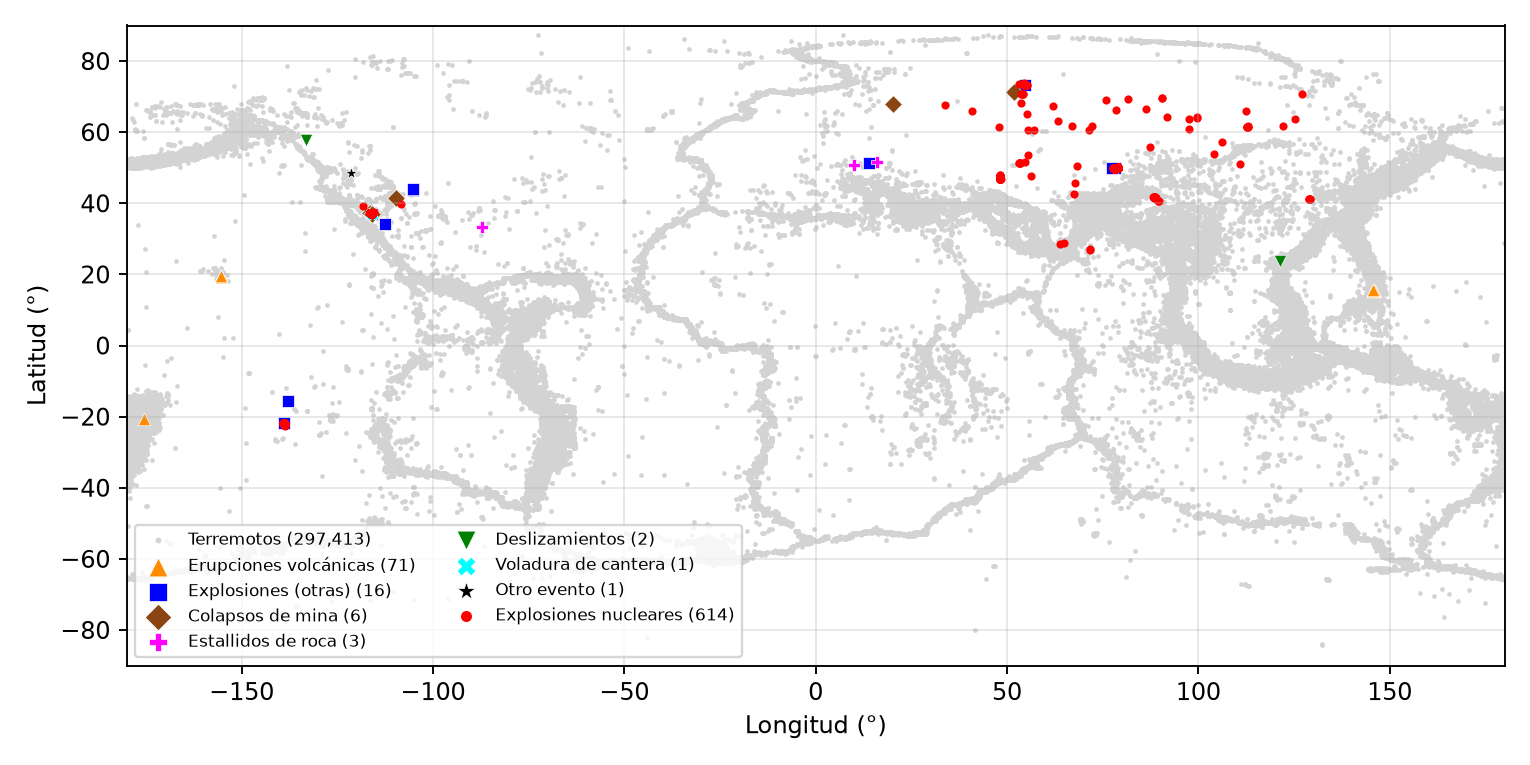
\includegraphics[width=0.92\textwidth]{figuras/catalogo.png}
\caption{Catálogo completo: las explosiones (rojo) se concentran en unos pocos polígonos de ensayo.}
\end{figure}

\subsection{Fundamentación teórica}
DBSCAN \cite{ester1996} define los grupos por densidad. Dado $\varepsilon$ y $v_{\min}$, un punto es central si su
vecindad de radio $\varepsilon$ contiene al menos $v_{\min}$ puntos; dos puntos centrales a distancia $\le\varepsilon$
pertenecen al mismo grupo (alcanzabilidad por densidad) y los puntos sin vecindad suficiente que no alcanza ningún punto
central son ruido. Con $v_{\min}=1$ todo punto es central y los grupos son las componentes conexas del grafo que une
los sismos a menos de $\varepsilon$; es equivalente al clustering jerárquico de enlace simple cortado a la altura $\varepsilon$.

Los epicentros están sobre la esfera, así que la distancia correcta es la ortodrómica. La fórmula de \emph{haversine}
\cite{sinnott1984},
\[
d = 2R\arcsin\sqrt{\sin^2\!\tfrac{\Delta\varphi}{2}+\cos\varphi_1\cos\varphi_2\sin^2\!\tfrac{\Delta\lambda}{2}},\qquad R=6371\ \text{km},
\]
es numéricamente estable para distancias pequeñas y está implementada en \texttt{sklearn.cluster.DBSCAN}
\cite{pedregosa2011} (\texttt{metric='haversine'}, con $\varepsilon$ expresado en radianes, $\varepsilon_{\mathrm{rad}}=\varepsilon_{\mathrm{km}}/R$).
Aquí el clustering solo agrupa por posición; el criterio físico (profundidad) es el que etiqueta cada grupo.

Como las clases están muy desbalanceadas (614 explosiones frente a casi 300\,000 terremotos), la exactitud no sirve: un
detector que nunca marcase nada tendría un 99,8\,\% de aciertos. Se usan la precisión $P=\mathrm{TP}/(\mathrm{TP}+\mathrm{FP})$, el
recall $R=\mathrm{TP}/(\mathrm{TP}+\mathrm{FN})$ y su media armónica, $F_1=2PR/(P+R)=2\,\mathrm{TP}/(2\,\mathrm{TP}+\mathrm{FP}+\mathrm{FN})$.

\subsection{Método: cómo se detecta}
\begin{enumerate}
  \item \textbf{Agrupar por posición.} DBSCAN con distancia \emph{haversine} (distancia sobre la esfera; las
        coordenadas se pasan a radianes y el radio $\varepsilon$ se divide por el radio terrestre, 6371 km). Dos
        sismos pertenecen al mismo cluster si hay una cadena de sismos a menos de $\varepsilon$ km uno del siguiente.
  \item \textbf{Mirar la profundidad de cada cluster.} Se calcula la \emph{mediana} de profundidad de cada cluster
        (la mediana no se deja engañar por unos pocos valores atípicos).
  \item \textbf{Marcar como sospechosos} los clusters cuya mediana está en $[d_{\min}, d_{\max})$: casi en la
        superficie. Todos los sismos de un cluster sospechoso se marcan como \emph{detectados}.
  \item \textbf{Evaluar contra la etiqueta.} Acierto: detectado y explosión. Falso positivo (FP): detectado pero no
        explosión. Falso negativo (FN): explosión no detectada.
\end{enumerate}

El paso 1 es la función \texttt{agrupar}: pasa las coordenadas a radianes, divide $\varepsilon$ entre el radio terrestre y
llama a DBSCAN con la métrica \emph{haversine}.

\lstinputlisting[firstline=25,lastline=33,firstnumber=25,caption={\texttt{agrupar}: DBSCAN con distancia haversine.},label={lst:agrupar}]{../problemas/2_Nuclear/nukeDBSCAN_arnau.py}

Los pasos 2 y 3 son \texttt{nukeDBSCAN}: la mediana de profundidad de cada cluster y la selección de los que caen en la ventana.

\lstinputlisting[firstline=36,lastline=48,firstnumber=36,caption={\texttt{nukeDBSCAN}: clusters sospechosos por la mediana de profundidad.},label={lst:nukedbscan}]{../problemas/2_Nuclear/nukeDBSCAN_arnau.py}

El paso 4 es \texttt{errores}, que cuenta FP y FN con la etiqueta \texttt{tipo}.

\lstinputlisting[firstline=51,lastline=59,firstnumber=51,caption={\texttt{errores}: falsos positivos y falsos negativos.},label={lst:errores}]{../problemas/2_Nuclear/nukeDBSCAN_arnau.py}

\begin{figure}[H]
\centering
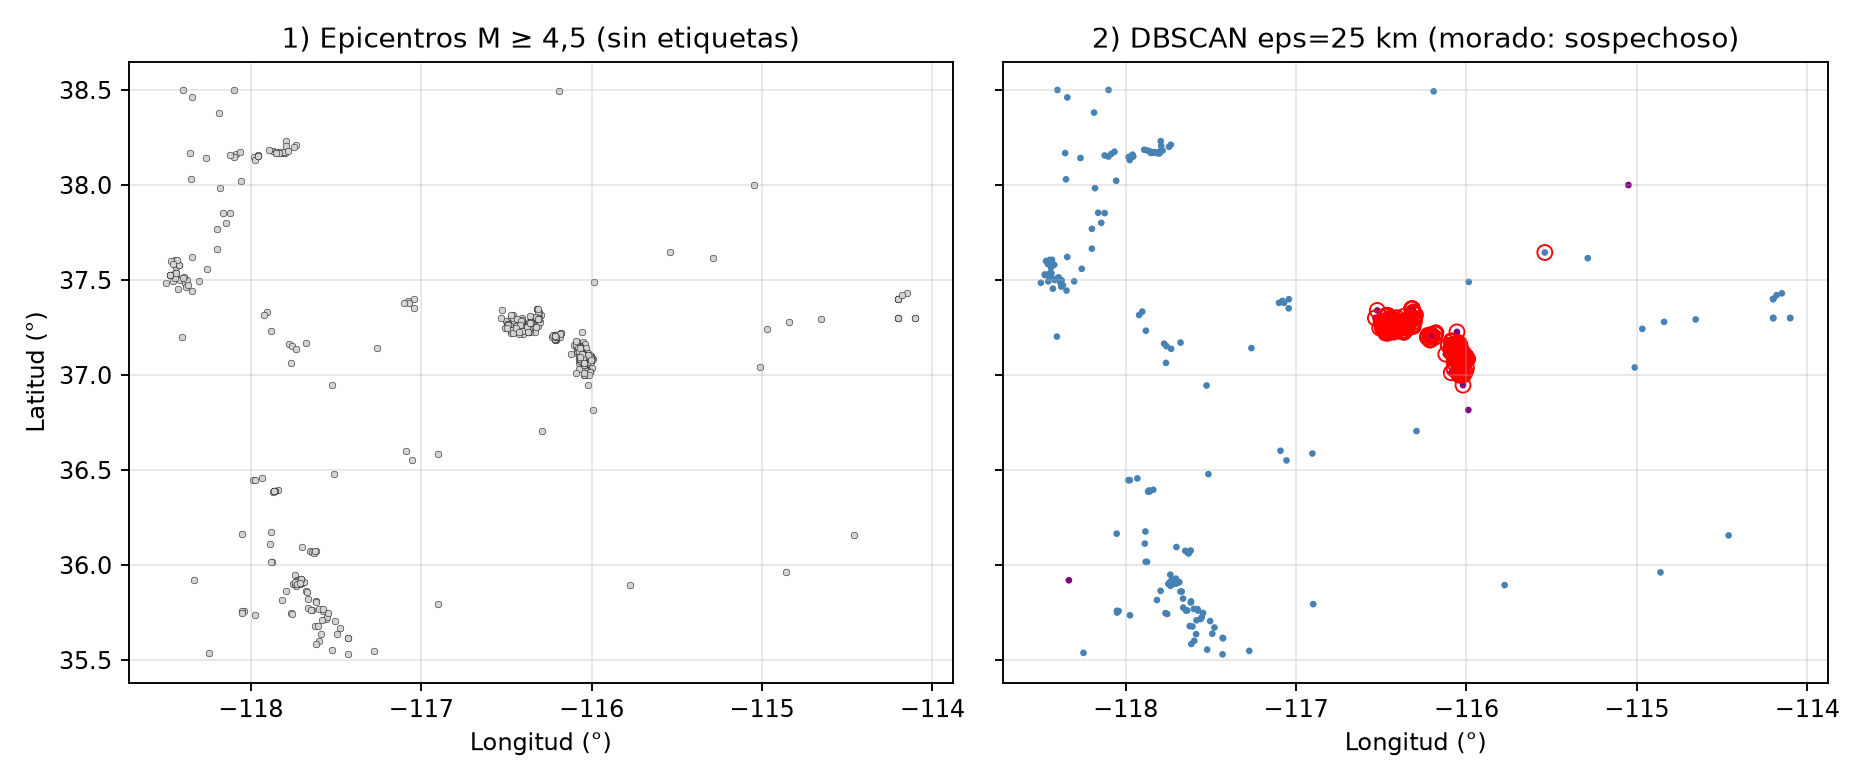
\includegraphics[width=0.95\textwidth]{figuras/deteccion_nevada.png}
\caption{Zoom en el polígono de Nevada. Izquierda: epicentros sin etiquetar. Derecha: clusters de DBSCAN; en morado,
los clusters sospechosos por profundidad; círculos rojos: explosiones reales (etiqueta USGS).}
\end{figure}

\begin{figure}[H]
\centering
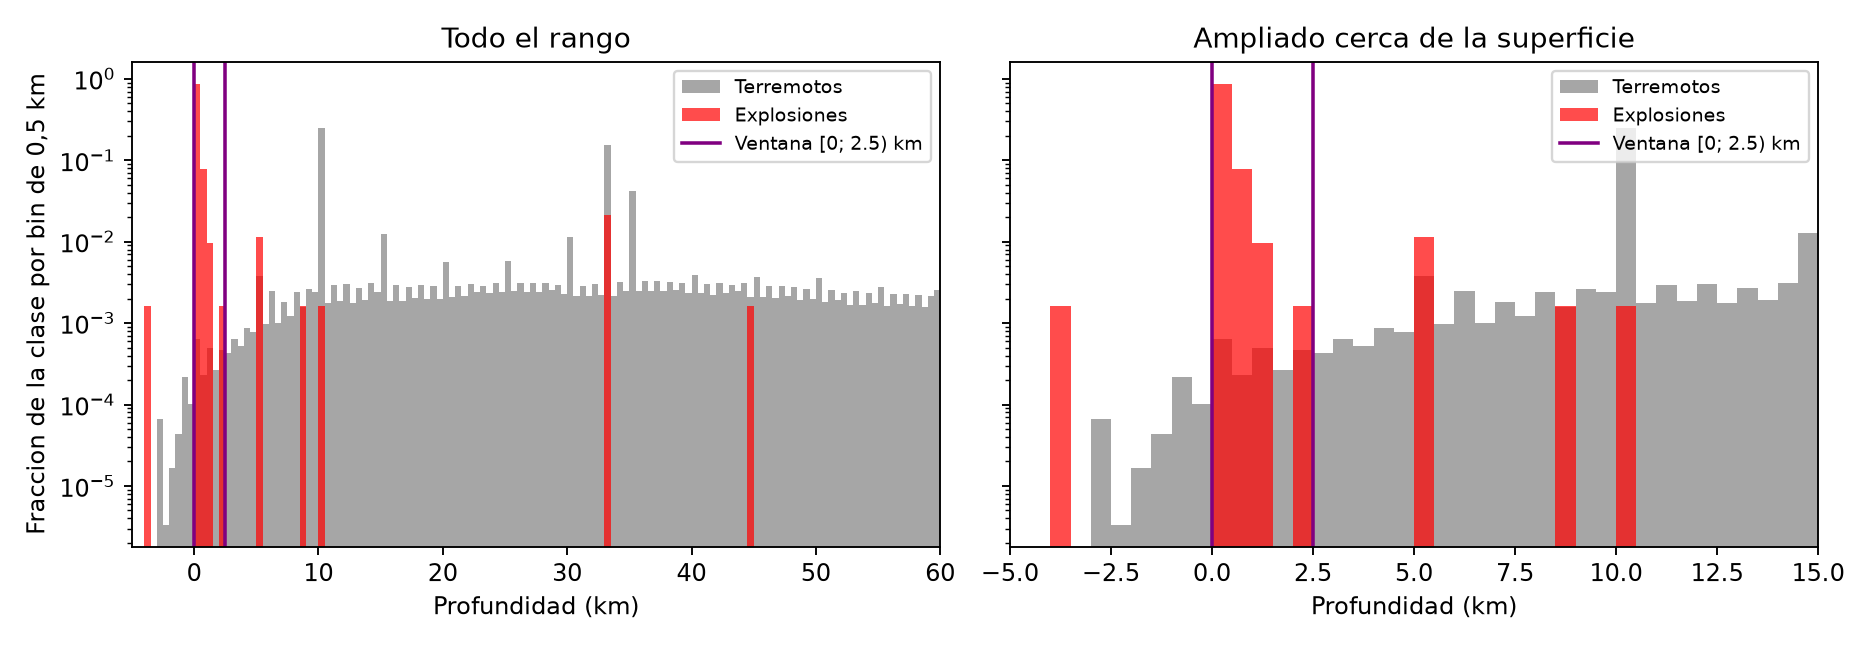
\includegraphics[width=\textwidth]{figuras/profundidad.png}
\caption{Distribución de profundidades: fracción de cada clase en bins de 0,5 km (escala logarítmica y mismo eje vertical), completa y ampliada cerca de la superficie. Las líneas moradas delimitan la ventana $[d_{\min}, d_{\max})$, que se aplica a la \emph{mediana} de cada cluster y no a cada sismo.}
\end{figure}

\subsection{Elección de parámetros}
Parámetros fijos: $\varepsilon=25$ km, $v_{\min}=1$, $d_{\min}=0$ y $d_{\max}=2{,}5$ km. Están en un único diccionario al
principio de \texttt{nukeDBSCAN\_arnau.py}, que \texttt{nukeval.py} importa.

\lstinputlisting[firstline=12,lastline=16,firstnumber=12,caption={\texttt{nukeDBSCAN\_arnau.py}: parámetros fijos.},label={lst:parametros}]{../problemas/2_Nuclear/nukeDBSCAN_arnau.py}

\begin{itemize}
  \item \textbf{Ventana de profundidad $[0;\,2{,}5)$ km:} criterio físico. Una explosión nuclear enterrada está a menos de
        unos pocos km de la superficie; los terremotos tectónicos están, en su mayoría, mucho más profundos.
  \item \textbf{$\varepsilon=25$ km:} del orden del tamaño de un polígono de ensayo. Es el valor con menos falsos positivos
        de los probados (5 a 100 km, ver la validación): con menos radio los terremotos superficiales quedan en grupos sueltos y
        con más radio los grupos de explosiones se funden con terremotos más profundos. Aquí sí se mira la etiqueta.
  \item \textbf{$v_{\min}=1$:} con $v_{\min}=3$ empeora (ver las limitaciones).
\end{itemize}
El script \texttt{nuke\_optimizar.py} (búsqueda de la ventana y de $\varepsilon$ por $F_1$) se probó, pero no se usa para
los parámetros finales: su óptimo, $[0;\,0{,}1)$ km, queda en el borde de su rejilla y aprovecha que el USGS registra con
profundidad exactamente $0{,}0$ km el 85\,\% de las explosiones (521 de 614) y solo 154 de 297\,513 eventos que no son
explosiones nucleares. Eso mide cómo cataloga el USGS y no la física. La tabla compara ventanas con $\varepsilon=25$ km.

\begin{table}[H]
\centering
\begin{tabular}{@{}lrrrr@{}}
\toprule
Ventana (km) & TP & FP & FN & $F_1$ \\
\midrule
$[0;\,0{,}1)$ (la que elegía el optimizador) & 585 & 58 & 29 & 0,931 \\
$[0;\,2{,}5)$ (usada) & 586 & 115 & 28 & 0,891 \\
$[0;\,5)$ & 587 & 363 & 27 & 0,751 \\
$[0;\,10)$ & 588 & 2\,897 & 26 & 0,287 \\
\bottomrule
\end{tabular}
\caption{Efecto de la ventana de profundidad ($\varepsilon=25$ km, $v_{\min}=1$).}
\end{table}

\subsection{Validación de $\varepsilon$ y estabilidad (\texttt{nukeval.py})}
Siguiendo el esquema de validación del temario (silueta, codo y estabilidad), \texttt{nukeval.py} evalúa $\varepsilon$
con $v_{\min}=1$ y la ventana $[0;\,2{,}5)$ km. Para cada $\varepsilon$ cuenta los clusters, calcula la silueta con
distancia haversine sobre una muestra de 2\,000 sismos (sin etiquetas) y los FP y FN (con etiquetas).

\lstinputlisting[firstline=18,lastline=46,firstnumber=18,caption={\texttt{nukeval.py}: silueta de unos clusters y tabla para cada $\varepsilon$ probado.},label={lst:val-eps}]{../problemas/2_Nuclear/nukeval.py}

La estabilidad compara los clusters del catálogo completo con los de cinco muestras aleatorias del 50\,\% mediante el ARI.

\lstinputlisting[firstline=59,lastline=70,firstnumber=59,caption={\texttt{nukeval.py}: estabilidad con el Adjusted Rand Index.},label={lst:val-ari}]{../problemas/2_Nuclear/nukeval.py}

\begin{table}[H]
\centering
\begin{tabular}{@{}rrrrr@{}}
\toprule
$\varepsilon$ (km) & Clusters & Silueta & FP & FN \\
\midrule
5 & 111\,117 & $0{,}01$ & 500 & 15 \\
10 & 44\,804 & $-0{,}18$ & 251 & 13 \\
25 & 11\,049 & $-0{,}45$ & 115 & 28 \\
40 & 5\,691 & $-0{,}43$ & 123 & 30 \\
50 & 4\,214 & $-0{,}50$ & 483 & 28 \\
100 & 1\,786 & $-0{,}51$ & 151 & 269 \\
\bottomrule
\end{tabular}
\caption{Validación de $\varepsilon$ (extracto; \texttt{nukeval.py} imprime 10 valores).}
\end{table}

\begin{figure}[H]
\centering
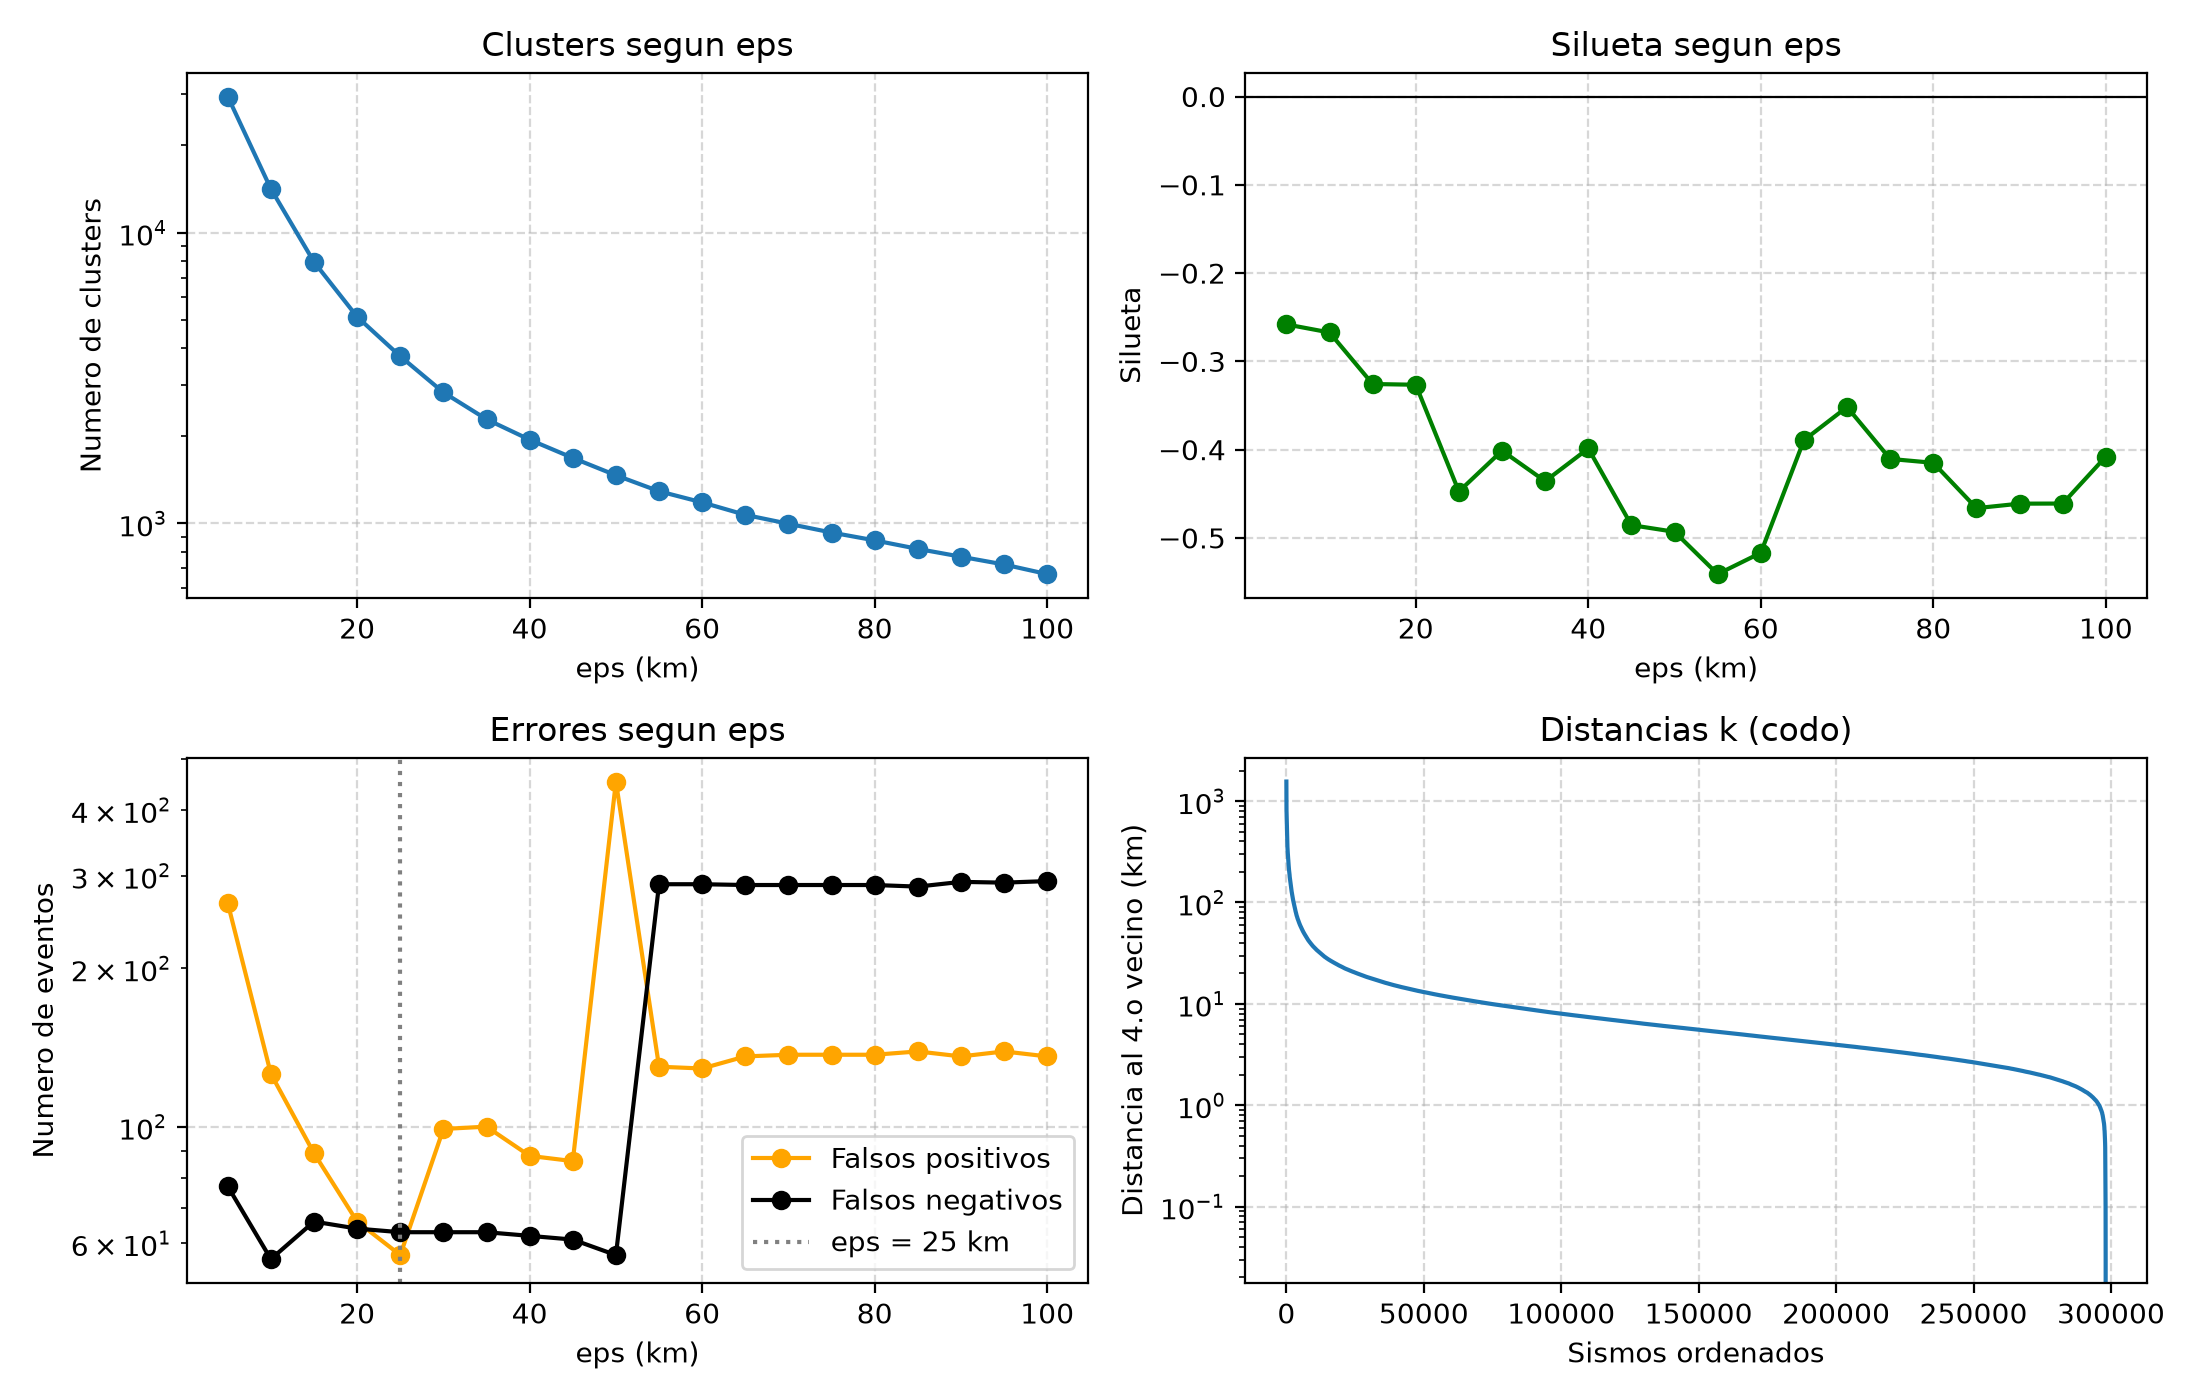
\includegraphics[width=\textwidth]{figuras/nukeval_eps.png}
\caption{Clusters, silueta y distancia al 4.º vecino (codo clásico de DBSCAN) frente a $\varepsilon$.}
\end{figure}

\begin{itemize}
  \item \textbf{La silueta no elige $\varepsilon$:} es negativa y decrece al aumentar $\varepsilon$. Con distancia por
        densidad, DBSCAN une cadenas alargadas de sismos y la silueta (que premia grupos compactos) lo penaliza. Tampoco el
        gráfico de distancias al 4.º vecino muestra un codo claro entre 20 y 30 km.
  \item \textbf{Lo que sí limita $\varepsilon$ es la profundidad:} los FP bajan al crecer $\varepsilon$ hasta un mínimo de 115 en
        25 km (con $\varepsilon$ pequeño muchos terremotos superficiales quedan en grupos sueltos); a partir de 40--50 km los
        grupos de explosiones se funden con terremotos más profundos: los FP suben a 483 con 50 km y los FN pasan de 28 a
        261 con 75 km, porque la mediana deja de ser superficial.
  \item \textbf{Estabilidad:} el ARI entre el clustering de todo el catálogo y el de una muestra aleatoria del 50\,\% (5
        semillas, $\varepsilon=25$ km) vale entre $0{,}54$ y $0{,}65$: moderado, porque al quitar sismos se rompen cadenas de DBSCAN.
\end{itemize}

\subsection{Resultados}
Con los parámetros fijos: 586 aciertos, 115 FP y 28 FN, es decir, precisión 83,6\,\%,
recall 95,4\,\% y $F_1=0{,}891$.

\begin{figure}[H]
\centering
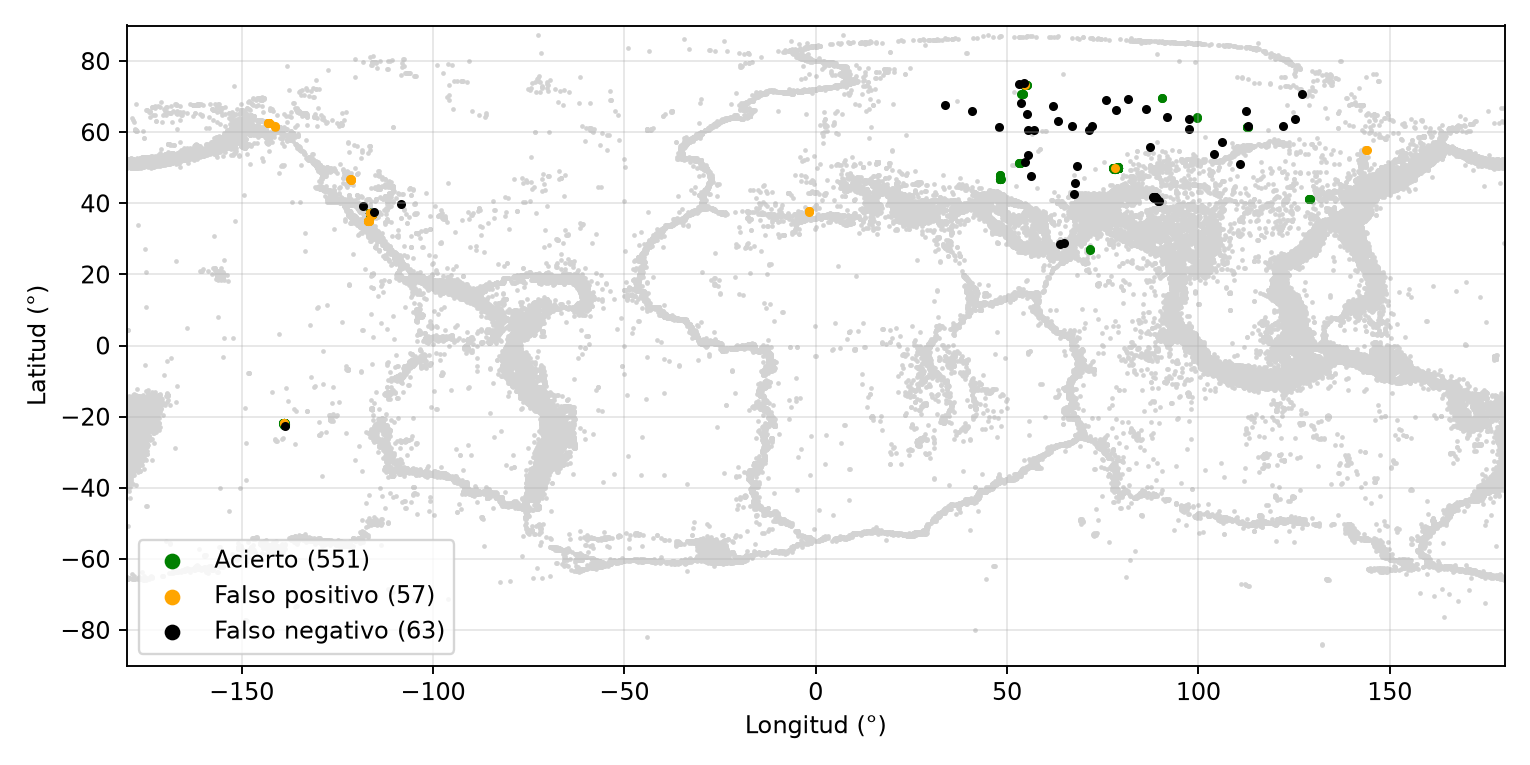
\includegraphics[width=0.92\textwidth]{figuras/resultado.png}
\caption{Resultado final: aciertos (verde), falsos positivos (naranja) y falsos negativos (negro).}
\end{figure}

\paragraph{Limitaciones y honestidad del resultado.}
\begin{itemize}
  \item \textbf{Con $v_{\min}=1$ no hay ruido:} cada sismo aislado forma su propio cluster. DBSCAN actúa aquí como un
        agrupador por proximidad encadenada, y la selección real la hace el filtro de profundidad. Con $v_{\min}=3$ el
        resultado empeora ($F_1=0{,}899$; FN = 69), porque muchas pruebas aisladas se perderían como «ruido».
  \item \textbf{Enfoque híbrido, no puramente no supervisado:} DBSCAN agrupa sin etiquetas y la ventana de profundidad es
        un criterio físico previo, pero $\varepsilon$ se ha escogido mirando el $F_1$ contra la etiqueta entre unos pocos
        valores, porque la silueta y el codo no lo determinan (ver la validación).
  \item \textbf{Generalización:} no hay un subconjunto de prueba separado: se ajusta y se evalúa en el mismo catálogo.
  \item \textbf{Convención del catálogo:} el 85\,\% de las explosiones figura con profundidad exactamente $0{,}0$ km.
        Una ventana más estrecha, $[0;\,0{,}1)$, daría $F_1=0{,}931$ pero mediría esa convención del USGS y no la física.
  \item \textbf{Falsos positivos:} terremotos muy superficiales (años 80 en Washington, California, Alaska) y otros
        eventos no sísmicos. De los 115 FP, 24 son de otro tipo: 16 \texttt{explosion}, 5 colapsos de mina, 1 voladura de cantera,
        1 estallido de roca y 1 deslizamiento; ninguna de las 71 erupciones volcánicas se marca. Si se descartasen los otros
        100 eventos no sísmicos (solo terremotos y explosiones nucleares), serían 91 FP y $F_1=0{,}908$. Algunas pruebas
        oficiales de Nevada figuran en el USGS como \texttt{earthquake}; ese error es de la etiqueta, no del método.
  \item \textbf{Sesgo de época:} no se usan el año ni el número de estaciones como variable, porque delatan la época
        del catálogo y no la física.
\end{itemize}

\subsection{Conclusiones}
\begin{itemize}
  \item Un clustering espacial sin etiquetas, combinado con la profundidad mediana de cada grupo, recupera el 95\,\% de las
        explosiones del catálogo ($F_1=0{,}891$) con 115 falsos positivos entre casi 300\,000 eventos.
  \item La señal útil es doble y física: repetición en los mismos polígonos de ensayo y profundidad casi nula.
  \item Líneas de mejora: elegir $\varepsilon$ en un subconjunto y evaluarlo en otro; añadir la magnitud y la forma de onda como variables; y usar la lista oficial
        DOE/NV-209 \cite{doe2015} en lugar de la etiqueta USGS para las pruebas de Nevada.
\end{itemize}

\subsection{Cómo reproducirlo}
\begin{enumerate}
  \item Crear el entorno: \texttt{python -m venv .venv} e instalar \texttt{requirements.txt}
        (numpy, pandas, matplotlib, scikit-learn, plotly).
  \item Opcional: \texttt{python problemas/2\_Nuclear/nukedatos.py} descarga del USGS el catálogo
        (\texttt{sismos\_usgs\_M45\_1951\_2025.csv}) a \texttt{datos/}; si el archivo ya existe, no hace nada.
  \item \texttt{python problemas/2\_Nuclear/nukeDBSCAN\_arnau.py} (se puede lanzar desde cualquier carpeta). Imprime FP y FN
        del run con los parámetros fijos y escribe \texttt{globo.html} (globo interactivo con 4 vistas, funciona sin internet).
  \item \texttt{python problemas/2\_Nuclear/nuke\_optimizar.py} reproduce la búsqueda por $F_1$ que se descartó
        (opcional; unos minutos).
  \item \texttt{python problemas/2\_Nuclear/nukeval.py} reproduce la validación de $\varepsilon$ y la estabilidad
        (unos 4 min) y guarda \texttt{nukeval\_eps.png} y \texttt{nukeval\_mapa.png}.
  \item Las figuras de este documento: \texttt{python docs/figuras\_nuclear.py}.
\end{enumerate}

% ==========================================
\section{Problema de Matías: agrupación de sismos y detección de anomalías}
% ==========================================
Material en \texttt{problemas/3\_Sismes\_Matias/} (README, código, datos e informe propio en catalán,
\texttt{informe\_sismes.tex}). Lo que sigue resume su \texttt{README.md} y su código; \emph{no he ejecutado su código ni he
comprobado sus resultados}.

\paragraph{Objetivo.} Segmentar los sismos globales del último mes con K-Means ($K=3$) según magnitud, profundidad,
latitud y longitud, para identificar patrones de subducción y actividad en los bordes de placa, y detectar eventos
excepcionales (alta magnitud o profundidad inusual) como anomalías.

\paragraph{Datos.} \texttt{earthquakes.csv}: 10\,174 eventos del catálogo USGS con cabecera estándar (\texttt{time, latitude,
longitude, depth, mag, \ldots}); el primero es del 15/10/2026.

\paragraph{Método.}
\begin{enumerate}
  \item Carga, reordenación de columnas y filtrado de registros incompletos o inválidos.
  \item Normalización $z$-score de las cuatro variables (media 0, desviación 1).
  \item K-Means con $K=3$.
  \item Anomalías: distancia euclídea media a los $k=5$ vecinos más próximos en el espacio normalizado; son anómalos
        los puntos más aislados.
\end{enumerate}

\paragraph{Validación.} Método del codo (WCSS), coeficiente de silueta y \emph{Adjusted Rand Index} (ARI) entre
inicializaciones distintas para medir la estabilidad; \texttt{validacio.py} también genera el mapa geográfico.

\paragraph{Reproducir.} \texttt{pip install -r requirements.txt} (pandas, numpy, scikit-learn, matplotlib), después
\texttt{python presentation\_matias.py} y \texttt{python validacio.py}. Hay versiones \texttt{*\_PANDAS.py} de ambos scripts.
Nota: el README nombra \texttt{problema\_matias.py}, que no existe en la carpeta, y los ficheros no siguen el formato
\texttt{<nemotécnico>\_<estudiante>.py} que pide el enunciado.

\pendiente{Matías: resultados (valor de $K$ elegido, silueta, ARI, anomalías encontradas) y su conclusión.}

\section{Problema de Martí: transcriptómica (RNA-seq)}
Material en \texttt{problemas/4\_RNAseq\_Marti/} (documento \texttt{EXPO CPIA - Clustering.docx}). Es por ahora un
\emph{plan}, sin código.

\paragraph{Objetivo.} Identificar módulos de genes co-expresados y detectar muestras anómalas en datos de RNA-seq con
aprendizaje no supervisado. La secuenciación mide la expresión de miles de genes a la vez y no hay etiquetas, porque no
se sabe de antemano qué genes funcionan juntos: es un problema de alta dimensionalidad.

\paragraph{Datos propuestos.} \texttt{scanpy.datasets.pbmc3k()} (2\,700 células sanguíneas humanas) o el conjunto UCI
\emph{Gene Expression Cancer RNA-Seq} de Kaggle (801 muestras de pacientes con distintos tipos de cáncer, en CSV).

\paragraph{Método previsto.}
\begin{itemize}
  \item Preprocesado: normalizar y aplicar logaritmo (los recuentos son asimétricos y dependen de la profundidad de secuenciación).
  \item Distancia: correlación en vez de euclídea, porque importa el patrón de expresión y no el valor absoluto.
  \item Clustering jerárquico con dendrograma: enlaces simple, medio y Ward, y cómo se corta el árbol.
  \item Validación sin etiquetas: silueta y codo para elegir $k$.
  \item Comparación con K-Means y DBSCAN.
  \item Isolation Forest para las muestras problemáticas.
  \item Conclusiones y limitaciones: maldición de la dimensionalidad, sensibilidad al preprocesado, datos sintéticos frente a reales.
\end{itemize}
\pendiente{Martí: código \texttt{.py}, resultados y figuras.}

\section{Problema de Uriel}
\pendiente{Uriel: título, datos, método, parámetros, resultados y código.}

\section{Problema de Uriel}
\pendiente{descripción detallada para reproducir el experimento: datos, método, parámetros, resultados, código.}

\section{Conclusiones del equipo}
\pendiente{comparativa de los cuatro problemas, qué algoritmo funcionó mejor y por qué.}

\clearpage
\thispagestyle{empty}
\null
\vspace*{\fill}
\begin{center}
{\fontsize{48}{58}\selectfont\bfseries Anexo}
\end{center}
\vspace*{\fill}
\clearpage

\section*{Anexo: código completo del problema de Arnau}
\addcontentsline{toc}{section}{Anexo: código completo del problema de Arnau}
Los tres programas del problema de las explosiones nucleares, tal como se ejecutaron. Cada sección del informe cita solo las
líneas que explican en ese punto.

\lstinputlisting[caption={\texttt{problemas/2\_Nuclear/nukedatos.py}: descarga del catálogo.},label={lst:anexo-datos}]{../problemas/2_Nuclear/nukedatos.py}

\lstinputlisting[caption={\texttt{problemas/2\_Nuclear/nukeDBSCAN\_arnau.py}: detección y globo interactivo.},label={lst:anexo-nuke}]{../problemas/2_Nuclear/nukeDBSCAN_arnau.py}

\lstinputlisting[caption={\texttt{problemas/2\_Nuclear/nukeval.py}: validación de $\varepsilon$ y estabilidad.},label={lst:anexo-val}]{../problemas/2_Nuclear/nukeval.py}

\begin{thebibliography}{9}
\bibitem{ester1996} Ester, M., Kriegel, H.-P., Sander, J., \& Xu, X. (1996). A density-based algorithm for discovering
clusters in large spatial databases with noise. \textit{Proc. 2nd Int. Conf. on Knowledge Discovery and Data Mining (KDD-96)}, 226--231.
\bibitem{pedregosa2011} Pedregosa, F., et al. (2011). Scikit-learn: Machine learning in Python. \textit{Journal of Machine
Learning Research}, 12, 2825--2830.
\bibitem{sinnott1984} Sinnott, R. W. (1984). Virtues of the haversine. \textit{Sky \& Telescope}, 68(2), 159.
\bibitem{usgs} U.S. Geological Survey. \textit{ANSS Comprehensive Earthquake Catalog (ComCat)}.
\url{https://earthquake.usgs.gov/data/comcat/}
\bibitem{doe2015} U.S. Department of Energy, Nevada Operations Office (2015). \textit{United States Nuclear Tests, July 1945
through September 1992}, DOE/NV-209 Rev. 16. \url{https://www.osti.gov/biblio/1351809}
\end{thebibliography}

\end{document}
